\documentclass{article}
\usepackage[utf8]{inputenc}
\usepackage[T1]{fontenc}
\usepackage[a4paper,top=3.5cm,bottom=3.5cm,left=2.5cm,right=2.5cm,marginparwidth=1.75cm]{geometry}
\usepackage{graphicx}
\usepackage[french,english]{babel} 
\usepackage{amsmath}
\usepackage{amssymb}
\usepackage{amsthm}
\usepackage{multicol}
\usepackage{fancyhdr}
\usepackage{booktabs}
\usepackage{hyperref}
\usepackage{cleveref}
\usepackage[labelfont=bf]{caption}
\usepackage{float}
%\usepackage[sorting=none]{biblatex}

\pagestyle{fancy}
\lhead{Ecole des Mines de Paris\hspace{1cm}---}
\chead{Trimestre Recherche}
\rhead{---\hspace{1cm}Année scolaire 2021-2022}

\setlength\parindent{0px}
\providecommand{\keywords}[1]{\textbf{\textit{Keywords ---}} #1}
\newcommand{\saut}{\vspace{10px}}

\begin{document}

\begin{center}
    \begin{Large}\textbf{Multi-task model to enhance short-term numerical weather predictions in Monaco}\end{Large}
    
    \vspace{1cm}
    \begin{large}\textbf{\underline{D.Castro$^a$}}\end{large}
    
    \vspace{0.5cm}
    a. \href{mailto:david.castro@mines-paristech.fr}{david.castro@mines-paristech.fr}
    \vspace{1cm}
\end{center}

\begin{abstract}
\vspace{5px}
\noindent Within the scope of the Energy Boat Challenge, this paper focuses on short-term solar and wind power 
prediction as a support to renewable-energy powered boats piloting. Considering both model-based numerical
predictions and \emph{in-situ} observations, the implemented models aim for correcting the former by
adding the latter's information.
Such strategy is first motivated by the will to combine numerical models' ability to provide valuable information
over many hours ahead and observations' accuracy.
Although machine and deep learning techniques meant to weather prediction
have recently led to a number of articles, a few take into account several types of inputs.
To that end, a simple baseline model was first investigated, revealing that
numerical predictions can easily be corrected that way and achieving satisfactory performances.
Then, as this work focuses on different tasks, multi-task neural networks were implemented in order to
benefit the most from the similarity between solar irradiance and wind predictions. Yet, none of them
managed to beat the linear models' results. It even appears that a simple autoregression on each feature
separately outputs almost as good results as the previous linear regression whereas it ignores numerical
predictions. As a matter of fact, in both cases, the term that seemingly provides the most valuable information
to the prediction is the most recent measurement of the targeted variable. Therefore, autoregression can be
considered the most efficient compromise between performances and the amount of data needed.
It reveals that the investigated models didn't succeed in capturing numerical predictions added value with respect
to \emph{in-situ} observations. To face that limit, the most relevant next step would be to work with data varying
with both time and space around the targeted location rather than simple timeseries. Doing so would allow
to deal with the numerical models geographical resolution explicitly and to provide a far more complete information
to the model.
\end{abstract}

\vspace{20px}

\keywords{Weather prediction, Multi-task neural network, NWP correction}

\section*{Notations}

NWP: Numerical Weather Predictions\\
\\
REAN: Reanalyses\\
\\
GHI: Global Horizontal Irradiance\\
\\
WS: Wind Speed\\
\\
WD: Wind Direction\\
\\
SHWW: Significant Height of Wind Waves\\
\\
For a feature F : $\mathrm F (t)$ is the measured value at time $t$, $\hat{\mathrm F}^\mathrm{NWP} (t + dt | t)$ is
the numerical prediction of F at time $t + dt$ knowing the history of the system
and $\hat{\mathrm F}^* (t + dt | t)$, the optimal data-driven obtained prediction of F at time $t + dt$ knowing the history.

\section{Introduction}

Accurate and precise solar and wind predictions are critical to the planning and use of renewable energies so that
power production can switch to dispatchable sources when strictly necessary. This concern has led to a large amount of
scientific articles. Many of them seek disruptive ways to predict future weather-related values including deep learning
\cite{zhong_multi-view_2021}.
Present work focuses on the usage of solar and wind power whitin the scope of a renewable energy-powered boats race
-- the Energy Boat Challenge organized each year since 2014 by the Monaco Yacht Club. Therefore, its goal is to provide
solar irradiance and wind speed and direction predictions that would enable either the pilotes to better anticipate
performances or people in charge to adapt the race's schedule. The quality of predictions being less critical than
when it comes to power generation and the purpose being specific, the models implemented are strictly limited to
local and short term prediction, namely over a few hours following present hour and at Monaco.

\saut

\emph{Zhong et al.} proposed an error correction multi-view deep learning network to predict
solar irradiance \cite{zhong_multi-view_2021}. The implemented model learns three different representations of the inputs 
to output one hour ahead irradiance. Similarly, \emph{Gulin et al.} built a predictor-corrector also meant to solar irradiance
forecast \cite{gulin_predictor-corrector_2015}. It tackles the lag and computational effort needed by numerical methods by implementing an observation-based model. It is composed of two parts: the predictor outputs raw
predictions of future solar irradiance as measurements become available while the corrector aims for transforming
the corrector's result to improve precision.

\saut

In both cases, the models are uniquely based on observations, that is to say they don't rely on a physical model.
They are pure supervised learning algorithms. By contrast, present work introduce a different approach consisting in
merging weather series from different types of sources : Numerical Weather Predictions (NWP) on the one hand and
local measurements on the other. Such method aims for improving the available numerical weather prediction by 
adding data from local and intentionally specific observations in near real-time. A few articles tackling the
enhancement of NWP can be found. For instance, \emph{Huang et al.} rely on the fusion of several numerical models to 
output more accurate predictions than each one of them \cite{huang_integrating_2012}. The issue consisting in the fusion 
of \emph{in-situ} observations is also widely documented since it is the starting point of NWP, called
\emph{data assimilation}: that stands for the computation
of the inital conditions of the forecast model. Thus, it is not a \emph{a posteriori} revision of the model's results but
a part of it. 

\saut

The following work rather answers to the question : can local observations help with NWP correction?
Its goal is to take advantage of several representations of the targeted variables to predict them as accurately as
possible. A series of NWP a few hours ahead are one of these representations. Contrary to the
others, it is able to provide information on the future. However, such information contains errors. That is why
the described strategy can be called NWP correction.
As revealed by \emph{Gulin et al.}, meteorological models complexity and their spatial resolution make NWP
correction an important issue \cite{gulin_predictor-corrector_2015}. This method will be conducted to
exploit as much as possible our problem's specificity either geographically or temporally.

\saut

Beyond the previous question, \emph{Linares-Rodriguez et al.} point out the relationships between
many meteorological variables \cite{linares-rodriguez_artificial_2013}. Their paper introduces a promising artificial
neural network predicting solar irradiance with high spatiotemporal resolution. Similarly to our strategy,
the model it investigates especially exploits different representations of the measured variables
-- satellite-based irradiance images -- to output accurate predictions.
That is why it uses a genetic algorithm to optimize selection of model input variables.
Therefore, considering the correlation between solar and wind power,
surface temperature and wind waves, our work raises the specific question: can
observation-based NWP correction benefit from a single model gathering all the tasks targeted,
a task being the prediction of one of the variables of interest, in comparison with
separate models for each of them? Multi-task models, predicting simultaneously solar irradiance and the wind vector,
were built to this end. \emph{Ruder} \cite{ruder_overview_2017} and \emph{Zang et al.} \cite{zhang_overview_2018}
introduce the key concepts of this type of networks.

\section{Method}

The issue is first to investigate NWP correction thanks to local measurements and secondly to evaluate
the effectiveness of a multi-task model to do so. Both questions need before all to implement baseline models
providing some elements of comparison to latter models and revealing whether even a simple model can
capture some useful information from local measurements to add to NWP.

\saut

Figure \ref{fig:Fig. 1} represent the general structure chosen for the investigated models. In general, for each
explanatory variable, they take
as input the series of the last $n$ measurements and a $2n$-long series of numerical predictions : the last $n$
predictions (from $t - n + 1$ to $t$) and the next $n$ ones (from $t + 1$ to $t + n$) when the targeted output is
values at time $t + 1, \dots, t + k$ where $k$ is the number of outputs of the task -- equal to $1$ on the figure.
It is clearly preferable to have $k \leq n$ and $n \leq 6$ considering the availability of NWP on live.
Measurements of the predicted variables at time $t + 1, \dots, t + k$ are also used as labels.

% Common model architecture explanations

\vspace{-30px}

\begin{figure}[H]
    \centering
    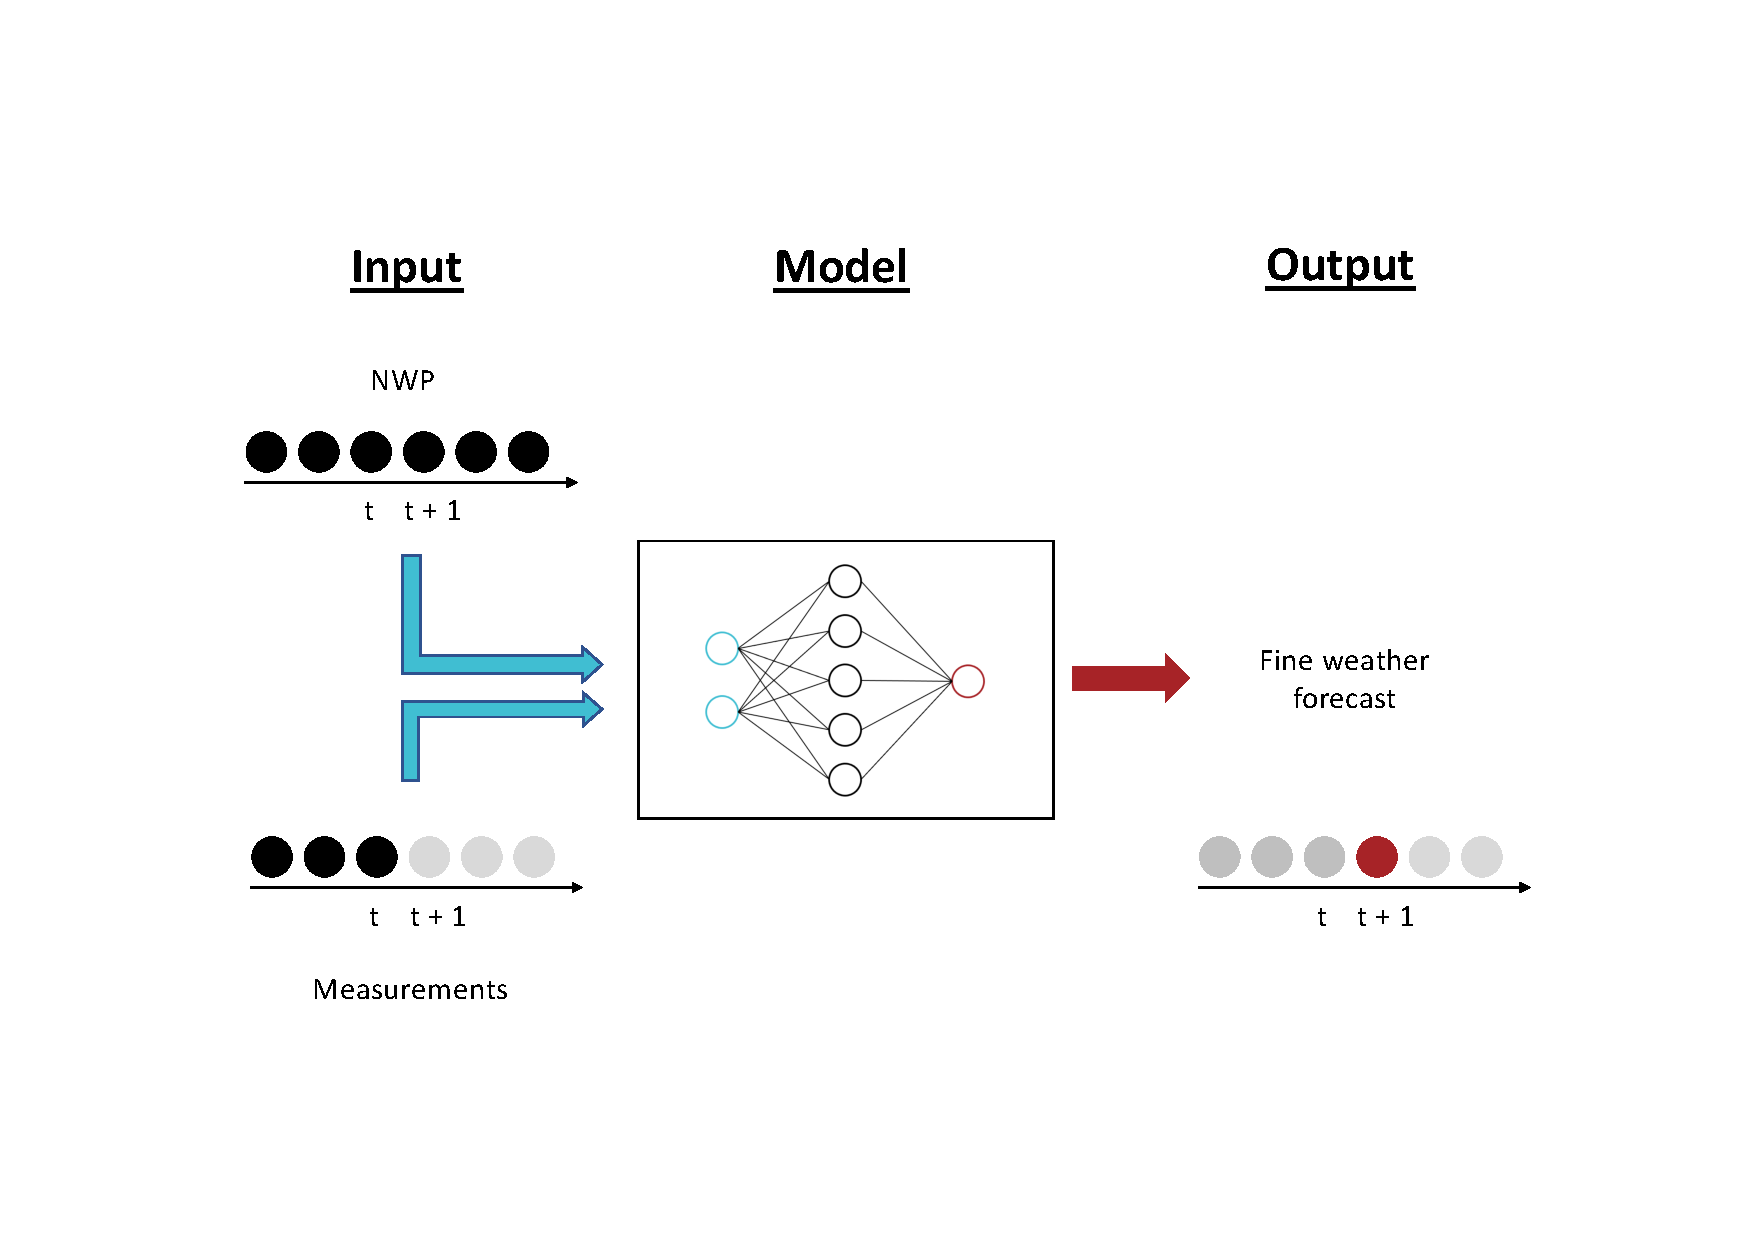
\includegraphics[width=\linewidth]{img/structure.pdf}
    \vspace{-30px}
    \caption{\textit{General architecture}}
   \label{fig:Fig. 1}
\end{figure}

\subsection*{Available data}

The implemented models focus on Global Horizontal Irradiance (GHI) as a measurement of solar power
and wind speed and wind direction as a measurement of wind power.
In particular, this work doesn't use the clear-sky index which consists in normalizing the GHI to make it
stationary over the day. It is often used because persistence over the clear-sky index allows good performances
as a baseline predictor. Its main drawback is that it excludes all night hours and would deprive the following models
of a lot of training samples which would still be interesting considering wind.
In order to avoid working with angles, wind inputs and outputs
take the form of the cartesian coordinates of the wind. Therefore, these are not direct measurements. Temperature will
also be considered but only as input. In other words, no model looks for predicting future temperature since it is
not directly responsible for the amount of renewable energy received, either solar or wind. Yet, it is still expected to
bear useful information to predict GHI or wind. GHI observations used are not direct measurements neither but
computed from satellite data. They are provided by the HelioClim project consisting in satellite-based measurements
of the reflection from the clouds and the ground enabling then to model reliably ground irradiance
\cite{blanc_helioclim_2011}. This method has led to effective GHI prediction models
\cite{linares-rodriguez_artificial_2013, mazorra_aguiar_use_2015}.

\saut

The numerical weather predictions used to evaluate the following models 
stem from the Europe Center for Medium-Range Weather Forecast (ECMWF), measurements come from a public
Météo-France buoy near Monaco and the SoDa database at the location of the buoy. Reanalyses from SoDa and
the Copernicus programme were also used to check data consistency. The quality control procedures (QCP) achieved
try to follow as much as possible the WMO standards \cite{organization_wmo_guidelines_2021}. Finally,
the considered data range from may to septembre each year between 2016 and 2021 and all have a one hour
time step. Focusing on such months allows to stick to the specific scope of the race and to expect the models
to exploit these specificities while learning.

\subsection*{Data consistency}

Initially, this work was also expected to take into account the significant height of wind waves (SHWW)
and their mean periods (MPWW).
They are indeed important factors concerning boat piloting. Moreover, wind waves were considered rather than swell
first because of geographical criteria and secondly because of their coupled dynamics with respect to wind, making it
a good candidate as part of a multi-task model. However, as illustrated in Figure \ref{shww}, the measurements, the
numerical predictions and the reanalyses were not consistent enough and thus could not be exploited. The two
latter logically fit well because by definition NWP takes part in the computation of reanalyses. Yet, the observations
don't match with them, being generally higher and quite uncorrelated except during peaks.
A possible explanations is that such measurements
are polluted by ship-generated waves, the buoy where the data come from being close to some crowded shipping
routes. Concerning the mean period of wind waves, the high quantization step size made it unusable neither.

\saut

\begin{figure}[H]
    \centering
    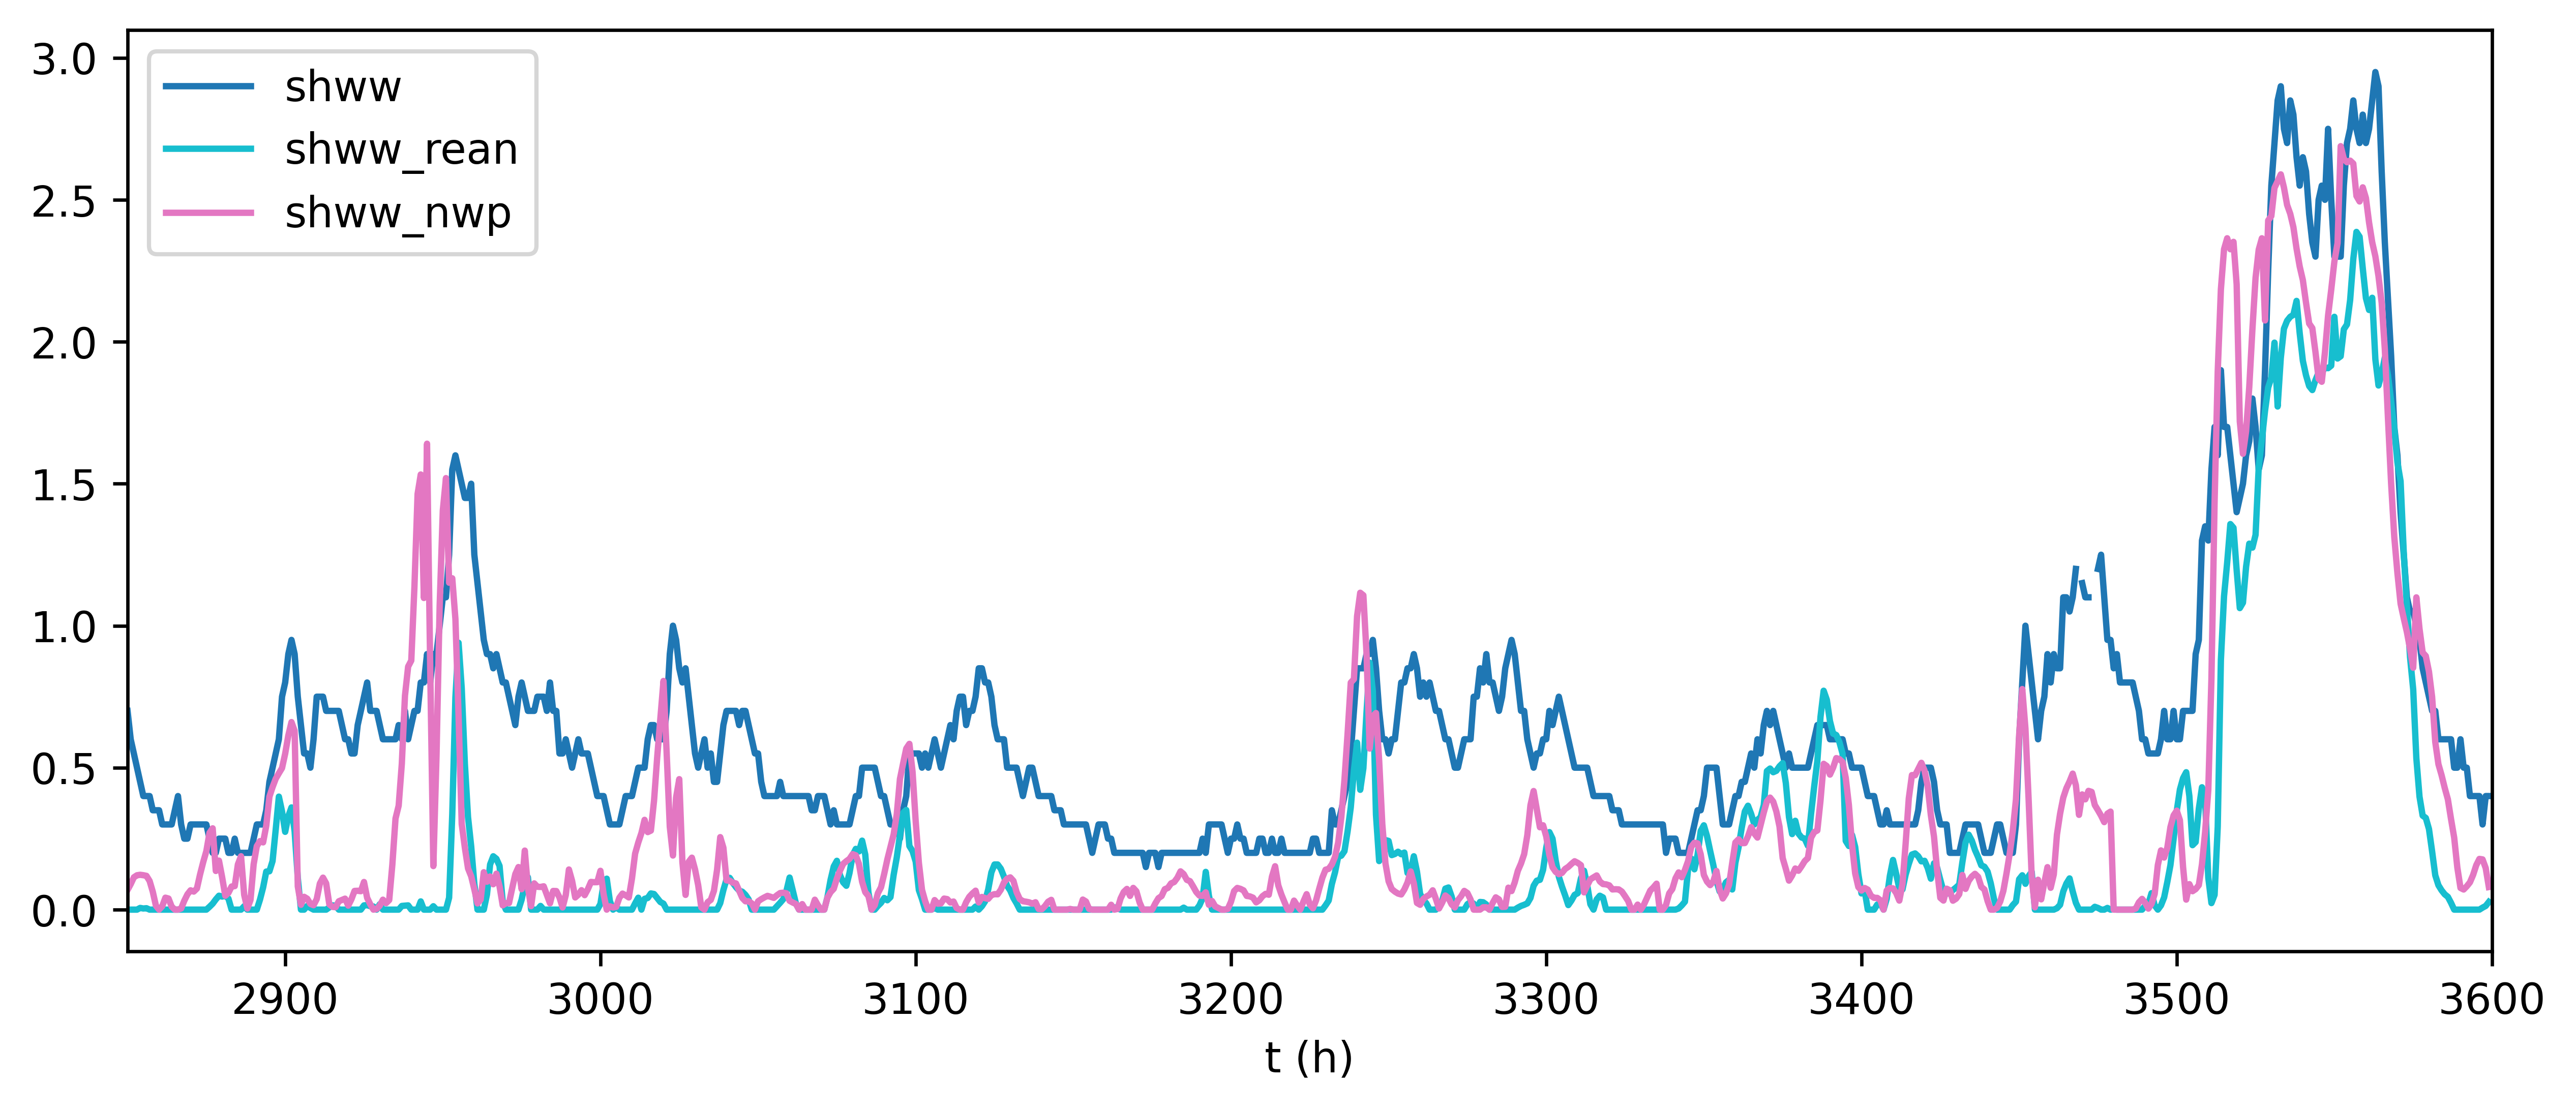
\includegraphics[width=.95\linewidth]{img/shww.png}
    \caption{\textit{Wind wave height}}
   \label{shww}
\end{figure}

On the contrary, as shown for wind speed on Figure \ref{ws_straight}, other features have high correlation levels.
For instance, the temperature correlation coefficient reaches $0.97$ and the GHI coefficient is equal to $0.98$.
These series still raised two QCP issues: filling the gaps in the data and controlling their self-consistencies.
Concerning the latter in particular, it is crucial to check for bounds and
maximal differences between successive values.
This was made following the criteria introduced by \emph{Espinar et al.} \cite{espinar_quality_nodate}.
Finally, one-hour-long gaps were filled using linear interpolation while reanalyses data were used
to complete bigger gaps. Such a choice was made first not to drop too much data -- one gap anywhere in
the data means a much wider loss in terms of training samples -- and secondly considering the low proportion
of concerned samples. For instance, between 2018 and 2020 included, each feature (except GHI) lacks about
200 samples over more than 10,000.

\saut

\begin{figure}[H]
    \centering
    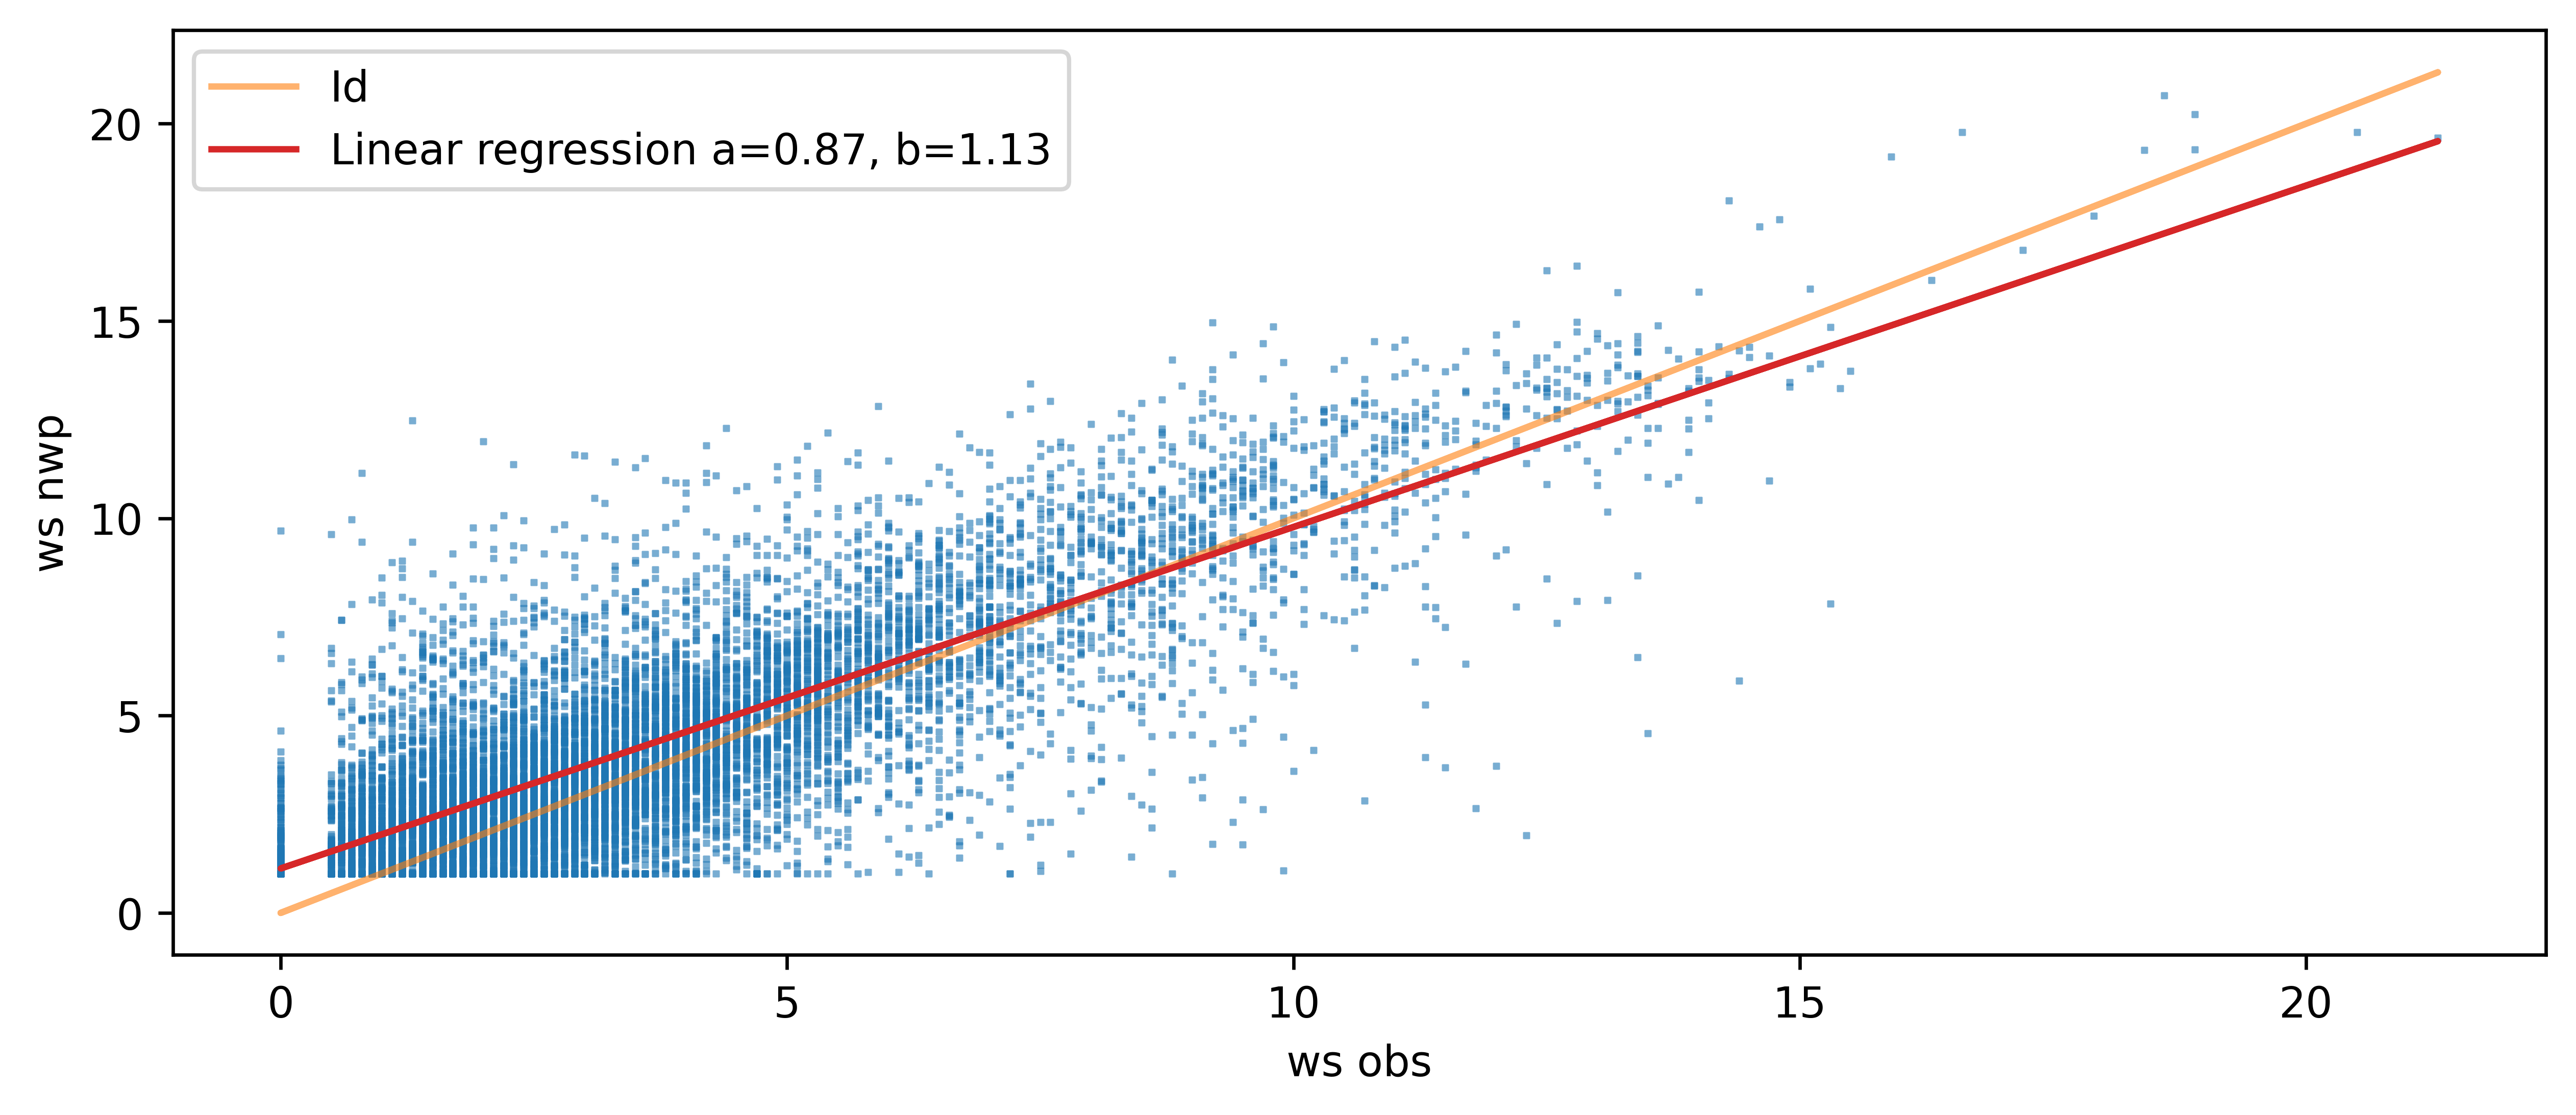
\includegraphics[width=\linewidth]{img/ws_compare.png}
    \caption{\textit{Wind speed regression}}
   \label{ws_straight}
\end{figure}

\subsection*{Baseline}

The implemented baseline is meant to assess two different key points : first, the performances allowed by a simple
model that more sophisticated models are to enhance and secondly, the way in which the different data
series individually participates in such performances.
To address these issues, the baselines mainly consist in single-output
linear regressions, that is to say outputing the value of a unique variable one hour ahead.
The choice of another machine learning algorithm -- regression random forest or persistence for instance -- have little
impact on targeted metrics.

\saut

In order to assess the impact of each part of the input on the quality of predictions, several architectures were investigated.
The simplest model built consists in an autoregression only based on past measurements of the targeted value.
It is meant to estimate the role of observations. A second basis corresponds to a linear regression taking as input
one hour ahead NWP and trained with measurements as labels. That stands for a first attempt to implement a
NWP corrector model. None of these two models follow the structure introduced in Figure \ref{fig:Fig. 1}.

\saut

Remaining baseline models take as input a series of $n$ past measurements, $n$ past NWP, the next $n$
numerical predictions per variable, for one or several variable -- including at least the targeted one -- and $n = 3$ or
$6$ typically, as explained in Figure \ref{fig:Fig. 1}. Several combination of explanatory variables were investigated.
In particular, to estimate how the knowledge of time (date and hour) change the quality of the predictions,
four artificial features were considered as input in some models : the one-year and one-day periodic sines and cosines.

\subsection*{Multi-task models}

In order to answer the second question raised by the introduction, several multi-task models were implemented.
They aim for revealing potential transfer learning between the predictions schemes of the different targeted variables.
Regarding the amount of data available, the first multi-task network built contains two or three shared layers and
one or two specific layers per predicted variable.

\newpage

As a multi-task model, its training minimizes only one metric. However, each task leads to one metric, chosen as
the Mean Squared Error (MSE). In order to solve such a multi-objective optimization problem, the chosen loss
function of the overall model L is a linear combination of the three losses. Let's note them
$\mathrm{MSE}_{\mathrm T}$
for each task T which can be T = GHI, $\mathrm W_{\mathrm x}$, $\mathrm W_{\mathrm y}$ for instance.
That solution corresponds to the multi-task models state-of-the-art.
Unfortunately, as the three losses can have different order of magnitude, defining
$L = \sum_{\mathrm T \in \mathrm{tasks}} \mathrm{MSE}_{\mathrm T}$ would cause an imbalanced training: the
higher the loss of one task, the more the training would focus on it, resulting in ignoring some of the others. To address
this issue, we have to normalize them by a default value leading us to take:

\saut

\[
	L := \sum_{\mathrm T \in \mathrm{tasks}}
	\frac{\mathrm{MSE}_{\mathrm T}}{\mathrm{MSE}^{\mathrm{baseline}}_{\mathrm T}}
\]

\vspace{-40px}

\begin{figure}[H]
    \centering
    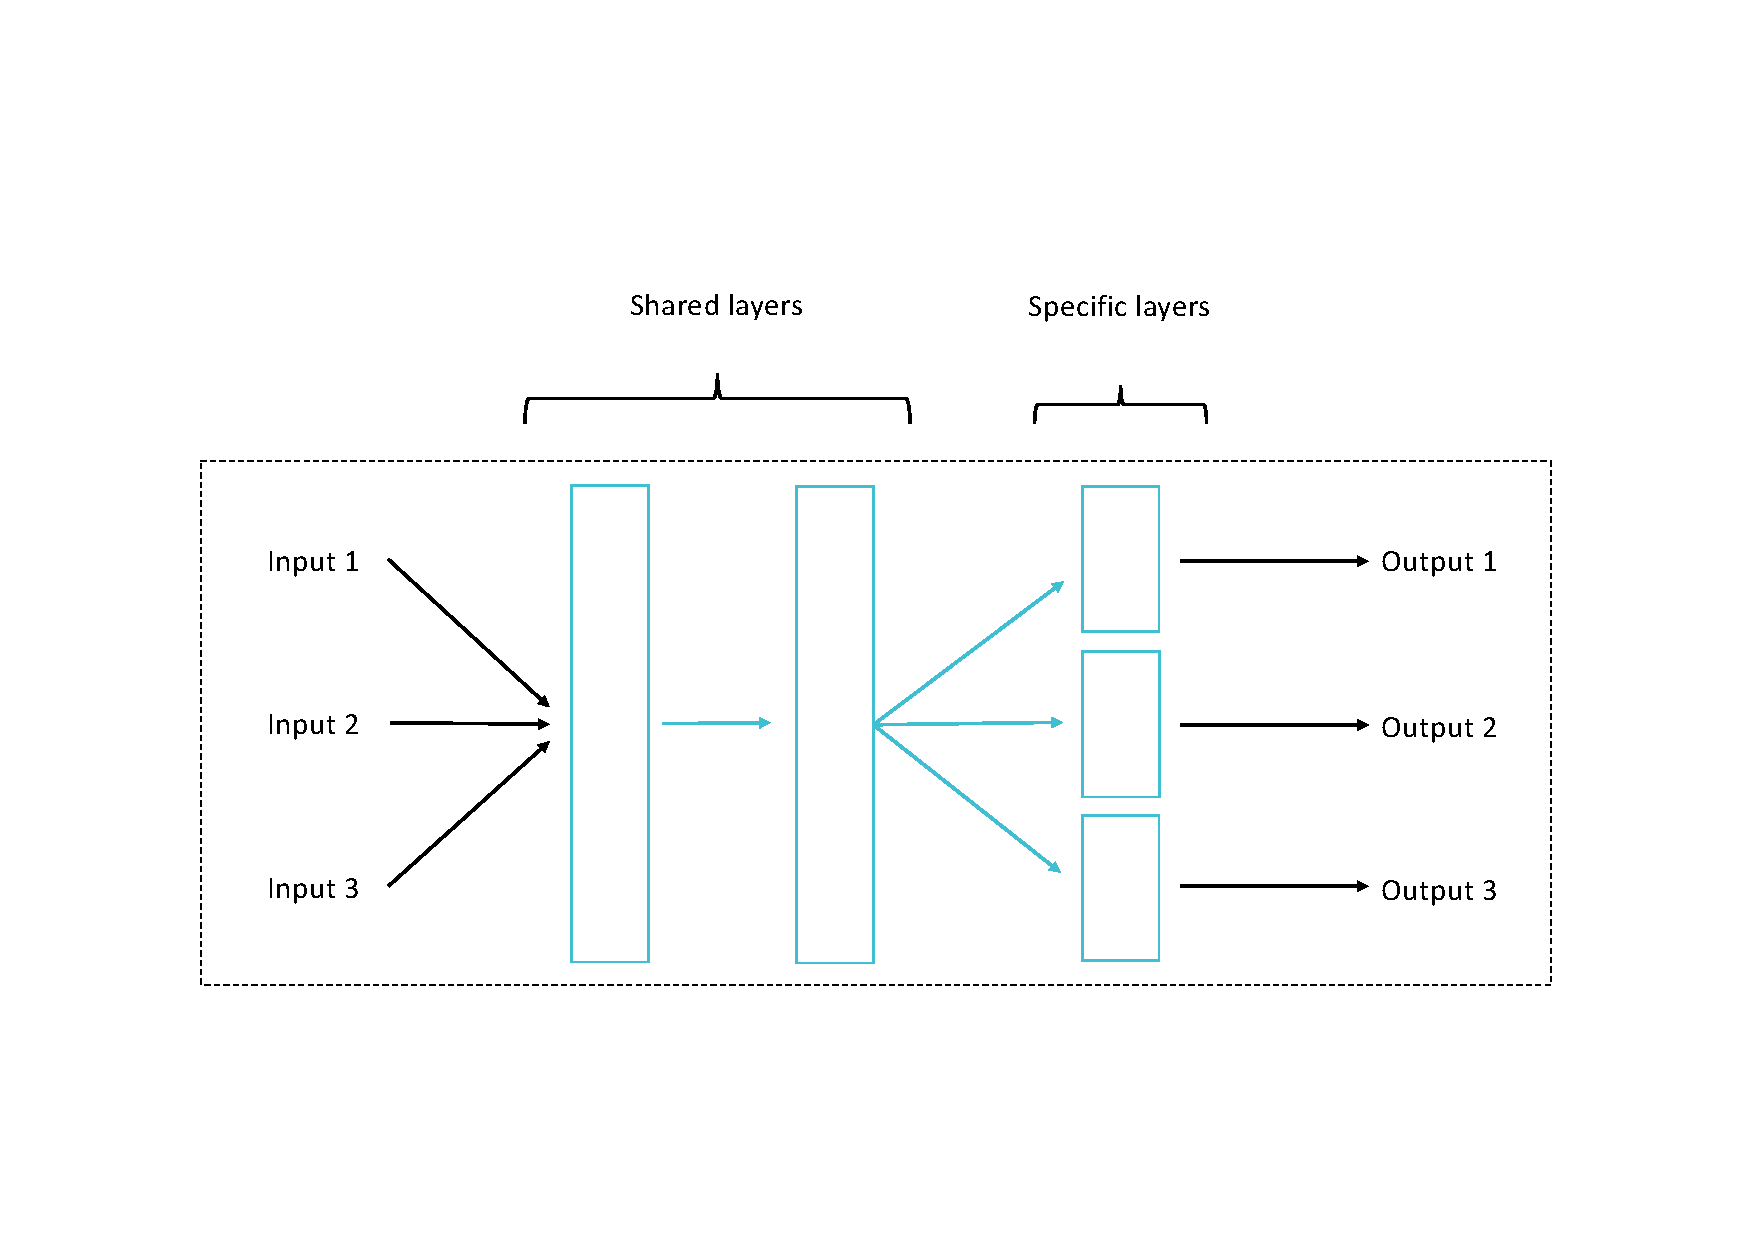
\includegraphics[width=.85\linewidth]{img/heads.pdf}
    \vspace{-30px}
    \caption{\textit{Multi-task network architecture}}
    \label{fig:Fig. 2}
\end{figure}

\vspace{-30px}

\begin{figure}[H]
    \centering
    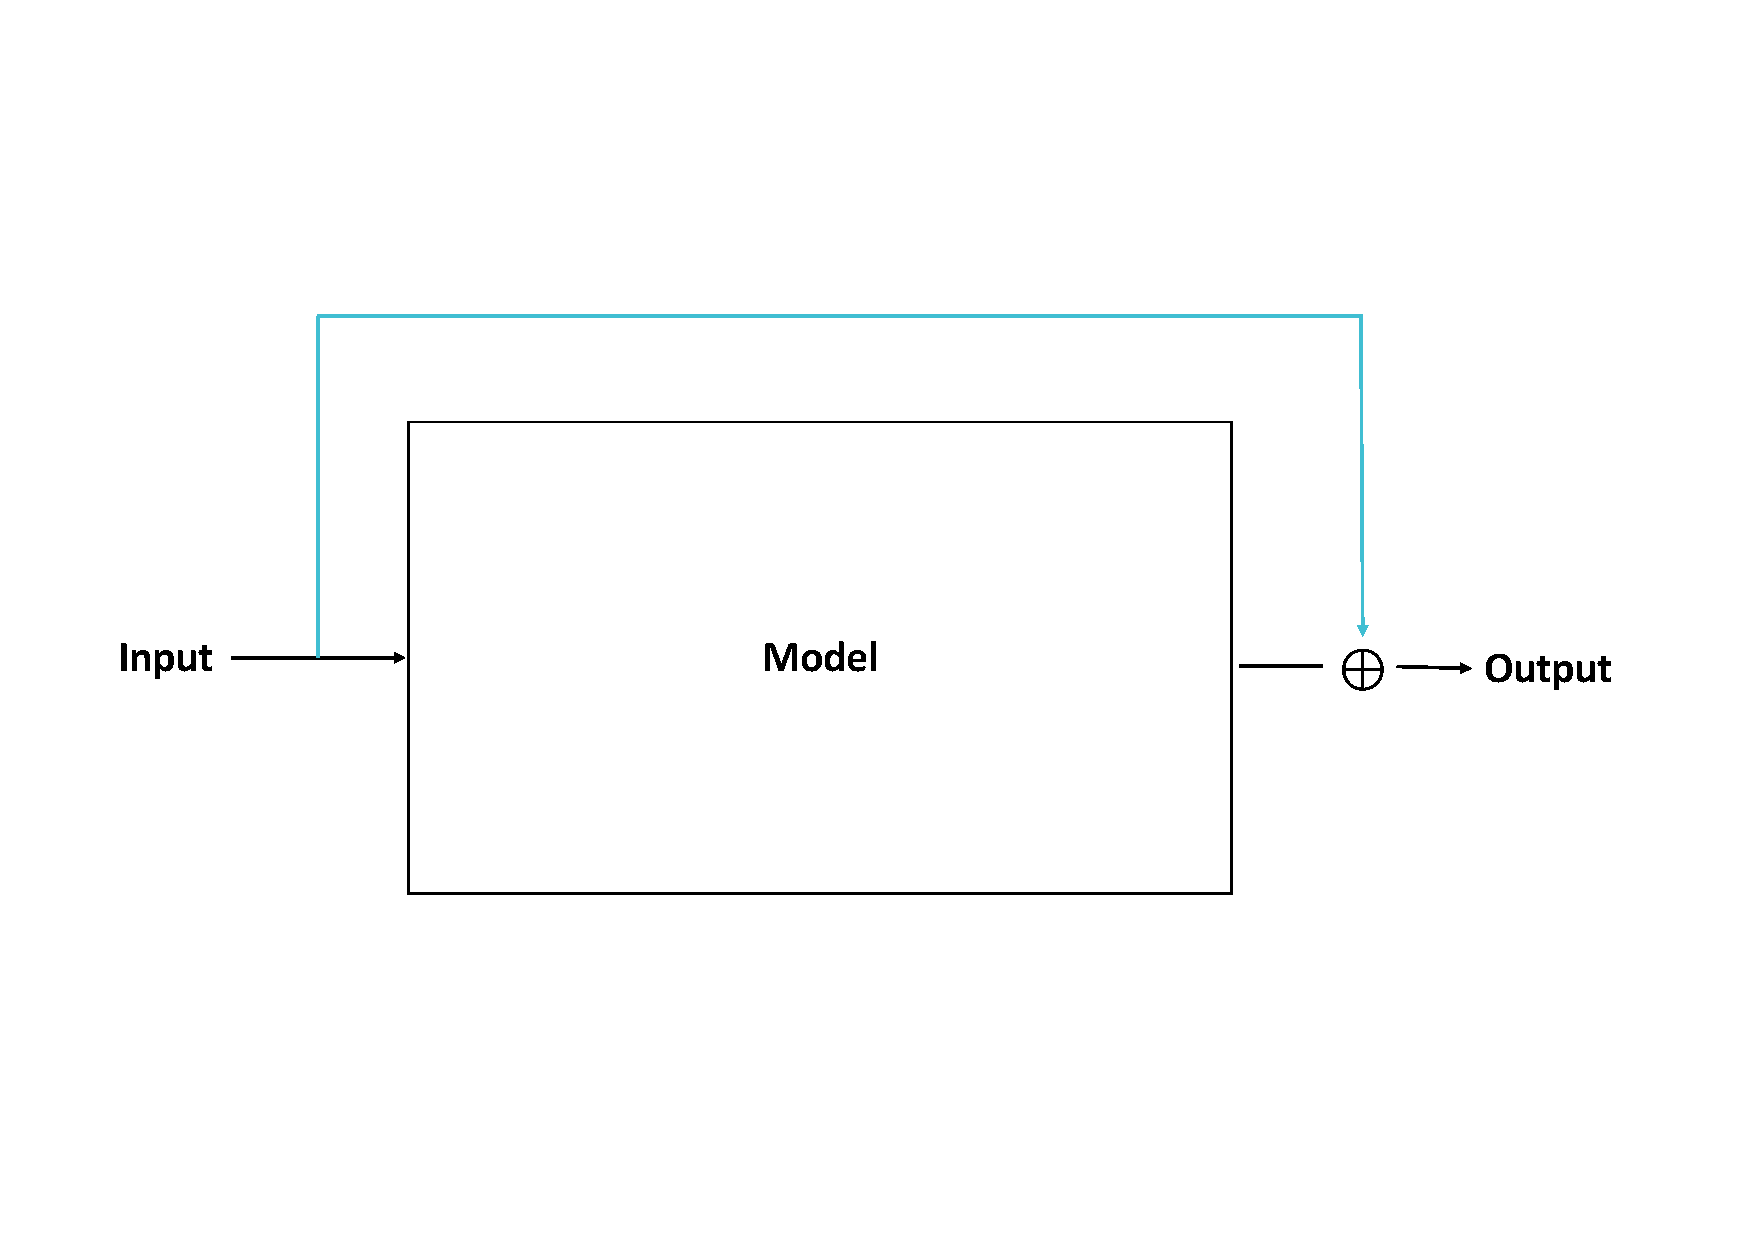
\includegraphics[width=.85\linewidth]{img/residual.pdf}
    \vspace{-30px}
    \caption{\textit{Residual network architecture}}
    \label{fig:Fig. 3}
\end{figure}

By considering the baseline MSE of the task as a normalization factor, having $\mathrm L_{\mathrm{pred}}$ at
the end of a prediction means that on quadratic average over the tasks, the model is
$\frac{\sqrt{\mathrm L_{\mathrm{pred}}}}{| \mathrm{tasks} | }$ times worse than the baselines.

\saut

The second model implemented is a multi-task \emph{ResNet}, which stands for residual network and consists in adding
the input to the output so that the model learns from the error between NWP and observations rather than observations
themselves directly. The corresponding architecture is represented Figure \ref{fig:Fig. 3} for a single-task model. Yet,
the principle is the same when it comes to a multi-task model. During the training, in the situation represented,
the model is equivalent to a standard network where the labels were replaced by the difference between the
labels and the input, which are the numerical prediction errors here.
The last multi-task network evaluated has convolutional shared layers so that it learns an abstract representation of the
data sent to each value-specific head. Its main advantage is take into account the structure of the data, that is to say
that it doesn't flatten the input matrix composed of different type of data series.

\section{Results and discussion}
\subsection*{Baseline}

The results of the baseline models are illustrated through wind speed predictions. Conclusions are very similar
for the other variables. Figure \ref{fig:Fig. 4} plots the results of a linear regression in dimension $1$, the explanatory
variable being NWP at time $t$ and the targeted output being the measured value at time $t + 1$. Analyzing both
the NWP empirical error distribution and the one of the
output of the model, such correction mainly removes the systematic bias.
Hence the need for adding past measurements to the input. This is what is done by the model whose results
are represented Figure \ref{fig:Fig. 5}.

% Continuing these explanations

\begin{figure}[H]
    \centering
    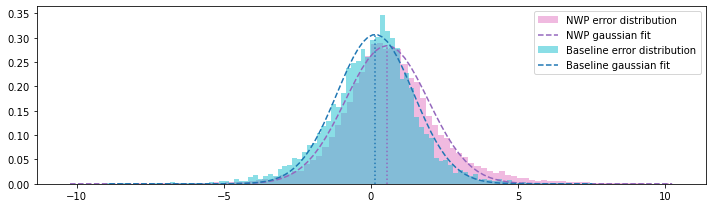
\includegraphics[width=\linewidth]{img/base.png}
    \caption{\textit{Wind speed simple regression result}}
    \label{fig:Fig. 4}
\end{figure}

This model corrects bias too but also reduces the standard deviation of the error distribution. In what follows,
as the errors approximately verify a normal distribution, the attention is mainly directed towards the standard
deviation. First, the bias $\varepsilon_0 = \mathbb E [ \varepsilon ]$ where $\varepsilon$ stands for the error,
needs much less information to be corrected: bias correction is achieved thanks to a simple addition.
Most of the investigated models thus remove it. Secondly, if $\hat \sigma$ is an estimate
of the standard deviation of $\varepsilon$ and $\hat \varepsilon_0$ is the empirical mean
of $\varepsilon$ -- which is the maximum-likelihood estimate of $\varepsilon_0$, we have:

\saut

\[
	\mathrm{RMSE} = \sqrt{\frac{1}{N} \sum_{i = 1}^N \varepsilon^2_i} \approx \sqrt{ \mathbb E [\varepsilon^2] }
	= \sqrt{\hat \sigma^2 + \hat \varepsilon^2_0}
\]

\begin{figure}[H]
    \centering
    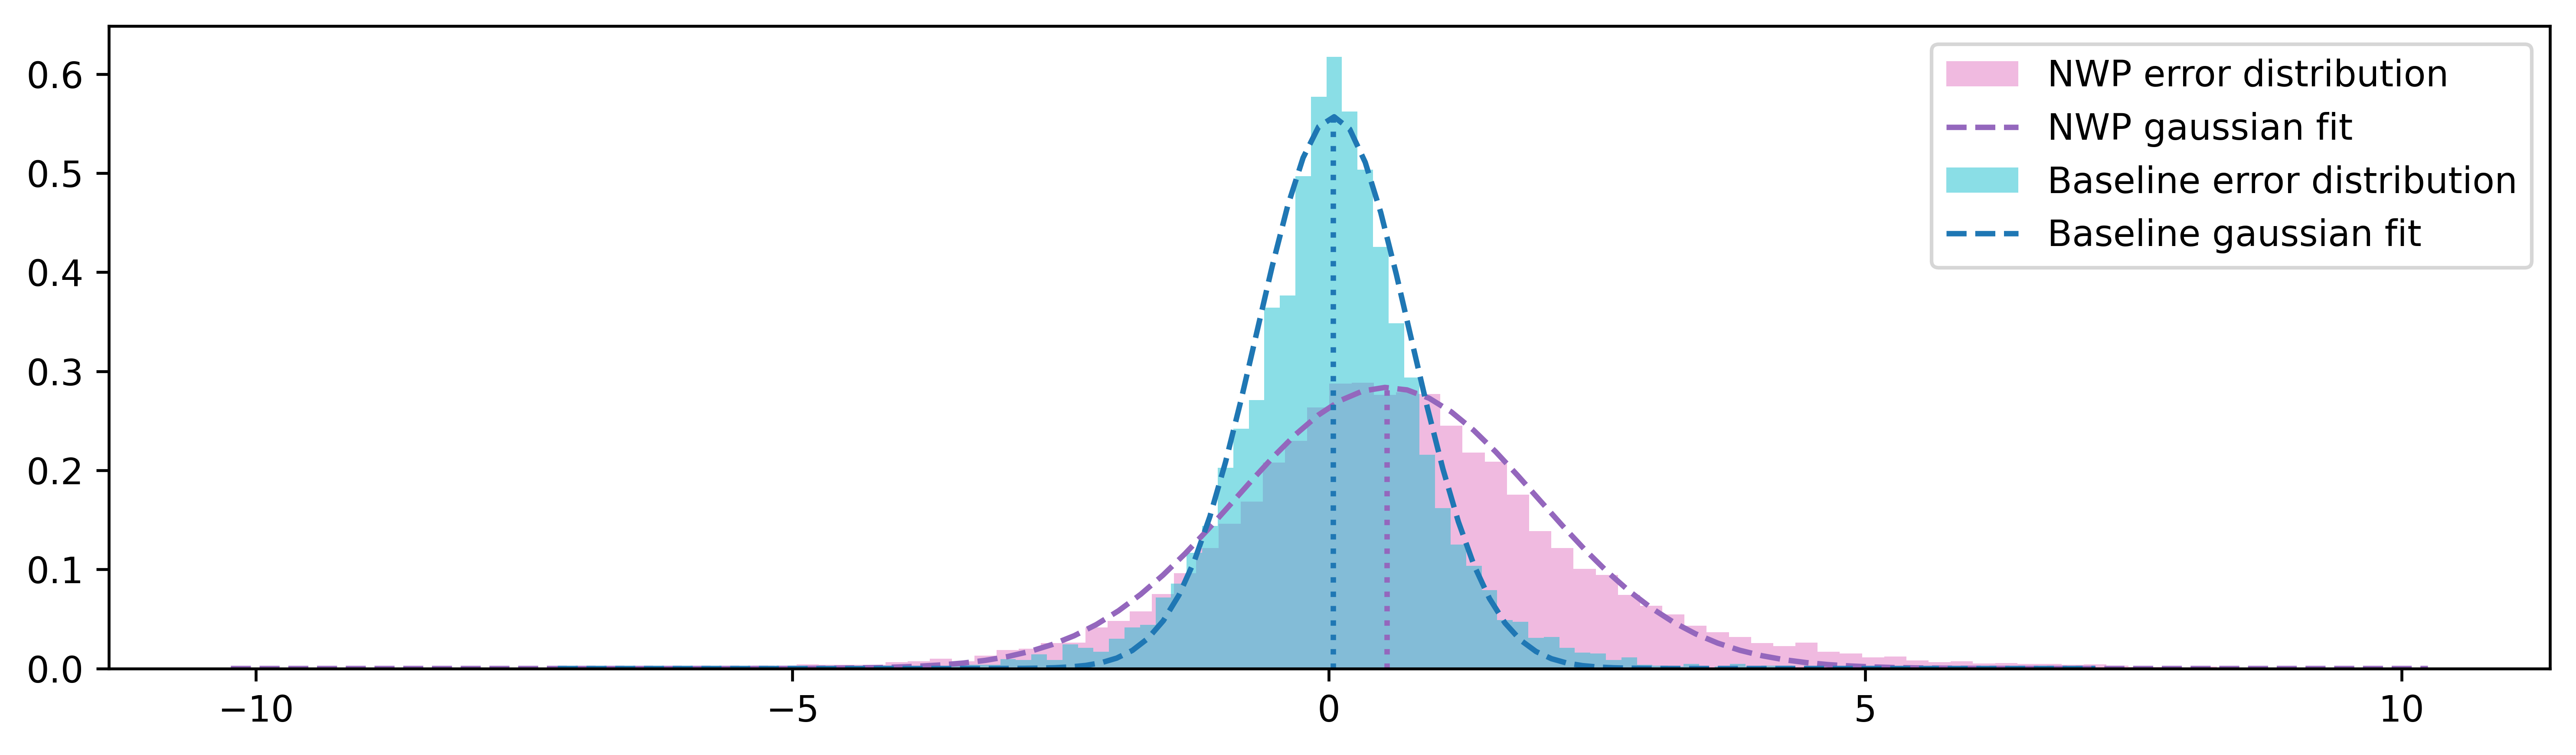
\includegraphics[width=\linewidth]{img/baseline.png}
    \caption{\textit{Wind speed baseline result}}
    \label{fig:Fig. 5}
\end{figure}

Therefore, when the a model's bias is indeed negligible, $\mathrm{RMSE} \approx \hat \sigma$.
The previous model is more performant regarding both criteria but its concrete interest
rather lies in the error distribution being sharper.

\saut

However, it is remarkable that an autoregression leads to almost as good results as the previous model, either
considering their empirical error distributions or their RMSE. Figure \ref{fig:Fig. 6} plots the coefficients associated with
each model in order to compare the hidden mechanisms behind such predictions. What appears is first that
the autoregression here is close to a persistence model in addition to bias correction: the predicted output is
approximately a linear function of the observation at time $t$. Secondly, the previous model, called \emph{baseline},
has quite similar coefficients as the autoregression. The main difference between the two series of coefficients
lies in the intercept: whereas the autoregression has a high one which stands for bias correction, the second model
has a very low intercept since the bias correction is rather computed from future NWP and past observations and NWP.
That reveals the interest of taking into account both measurements and short-term NWP. For the same reasons,
increasing the number of input timesteps $n$ or adding the date to the inputs has no significant effect on performances.

\saut

That is also what explains that an autoregressive scheme
is not effective for all variables: it leads to bad performances for the GHI
for instance. Yet, it is clear that such a linear regression over NWP and measurements, whose coefficients were
plotted, doesn't benefit the most from both series. It is therefore expected that a non-linear model reaches
better precision and even more a multi-task model which is able to exploit the similarity between the prediction of
the GHI and the wind.

% Almost persistence, that's why it works far worse for ghi --> a bit of luck here but not really interesting in general
% Interpretation (and other factors : n etc)

\saut

\begin{figure}[H]
    \centering
    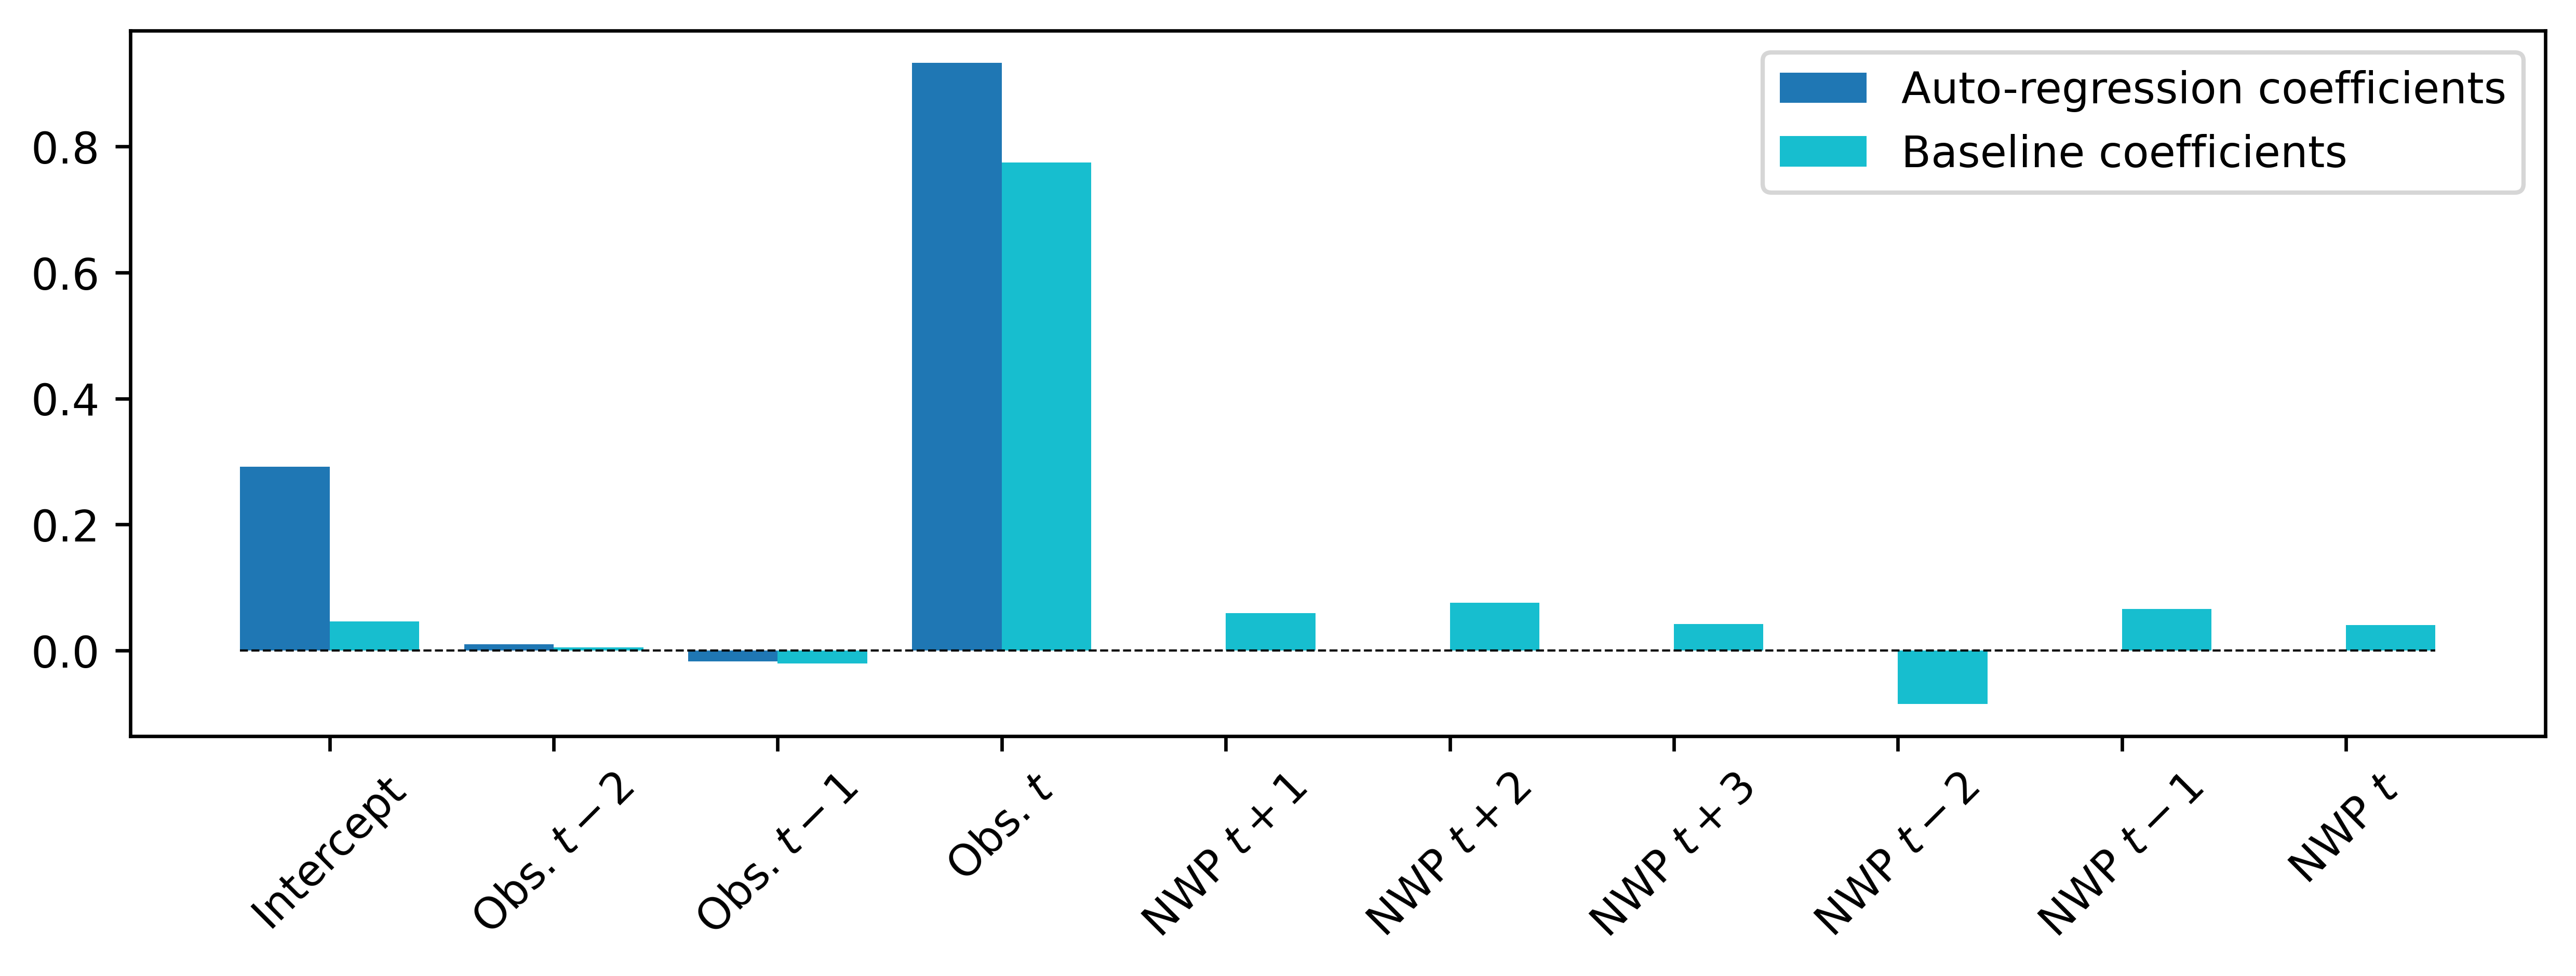
\includegraphics[width=\linewidth]{img/coef.png}
    \caption{\textit{Wind speed regression coefficients}}
    \label{fig:Fig. 6}
\end{figure}

\subsection*{Multi-task networks}

Each of the multi-task, the residual multi-task and the convolutional multi-task models actually
led to similar results as the baselines. The training generalizes well,
as shown on Figure \ref{fig:Res} and \ref{fig:Conv} and stop
when the loss approximately reaches the baseline performances.
As a matter of fact, the loss function were designed so that the models equal the baseline on quadratic average
over the tasks when the loss reaches 10.

\saut

\begin{figure}[H]
\centering
\begin{minipage}{.5\textwidth}
	\centering
	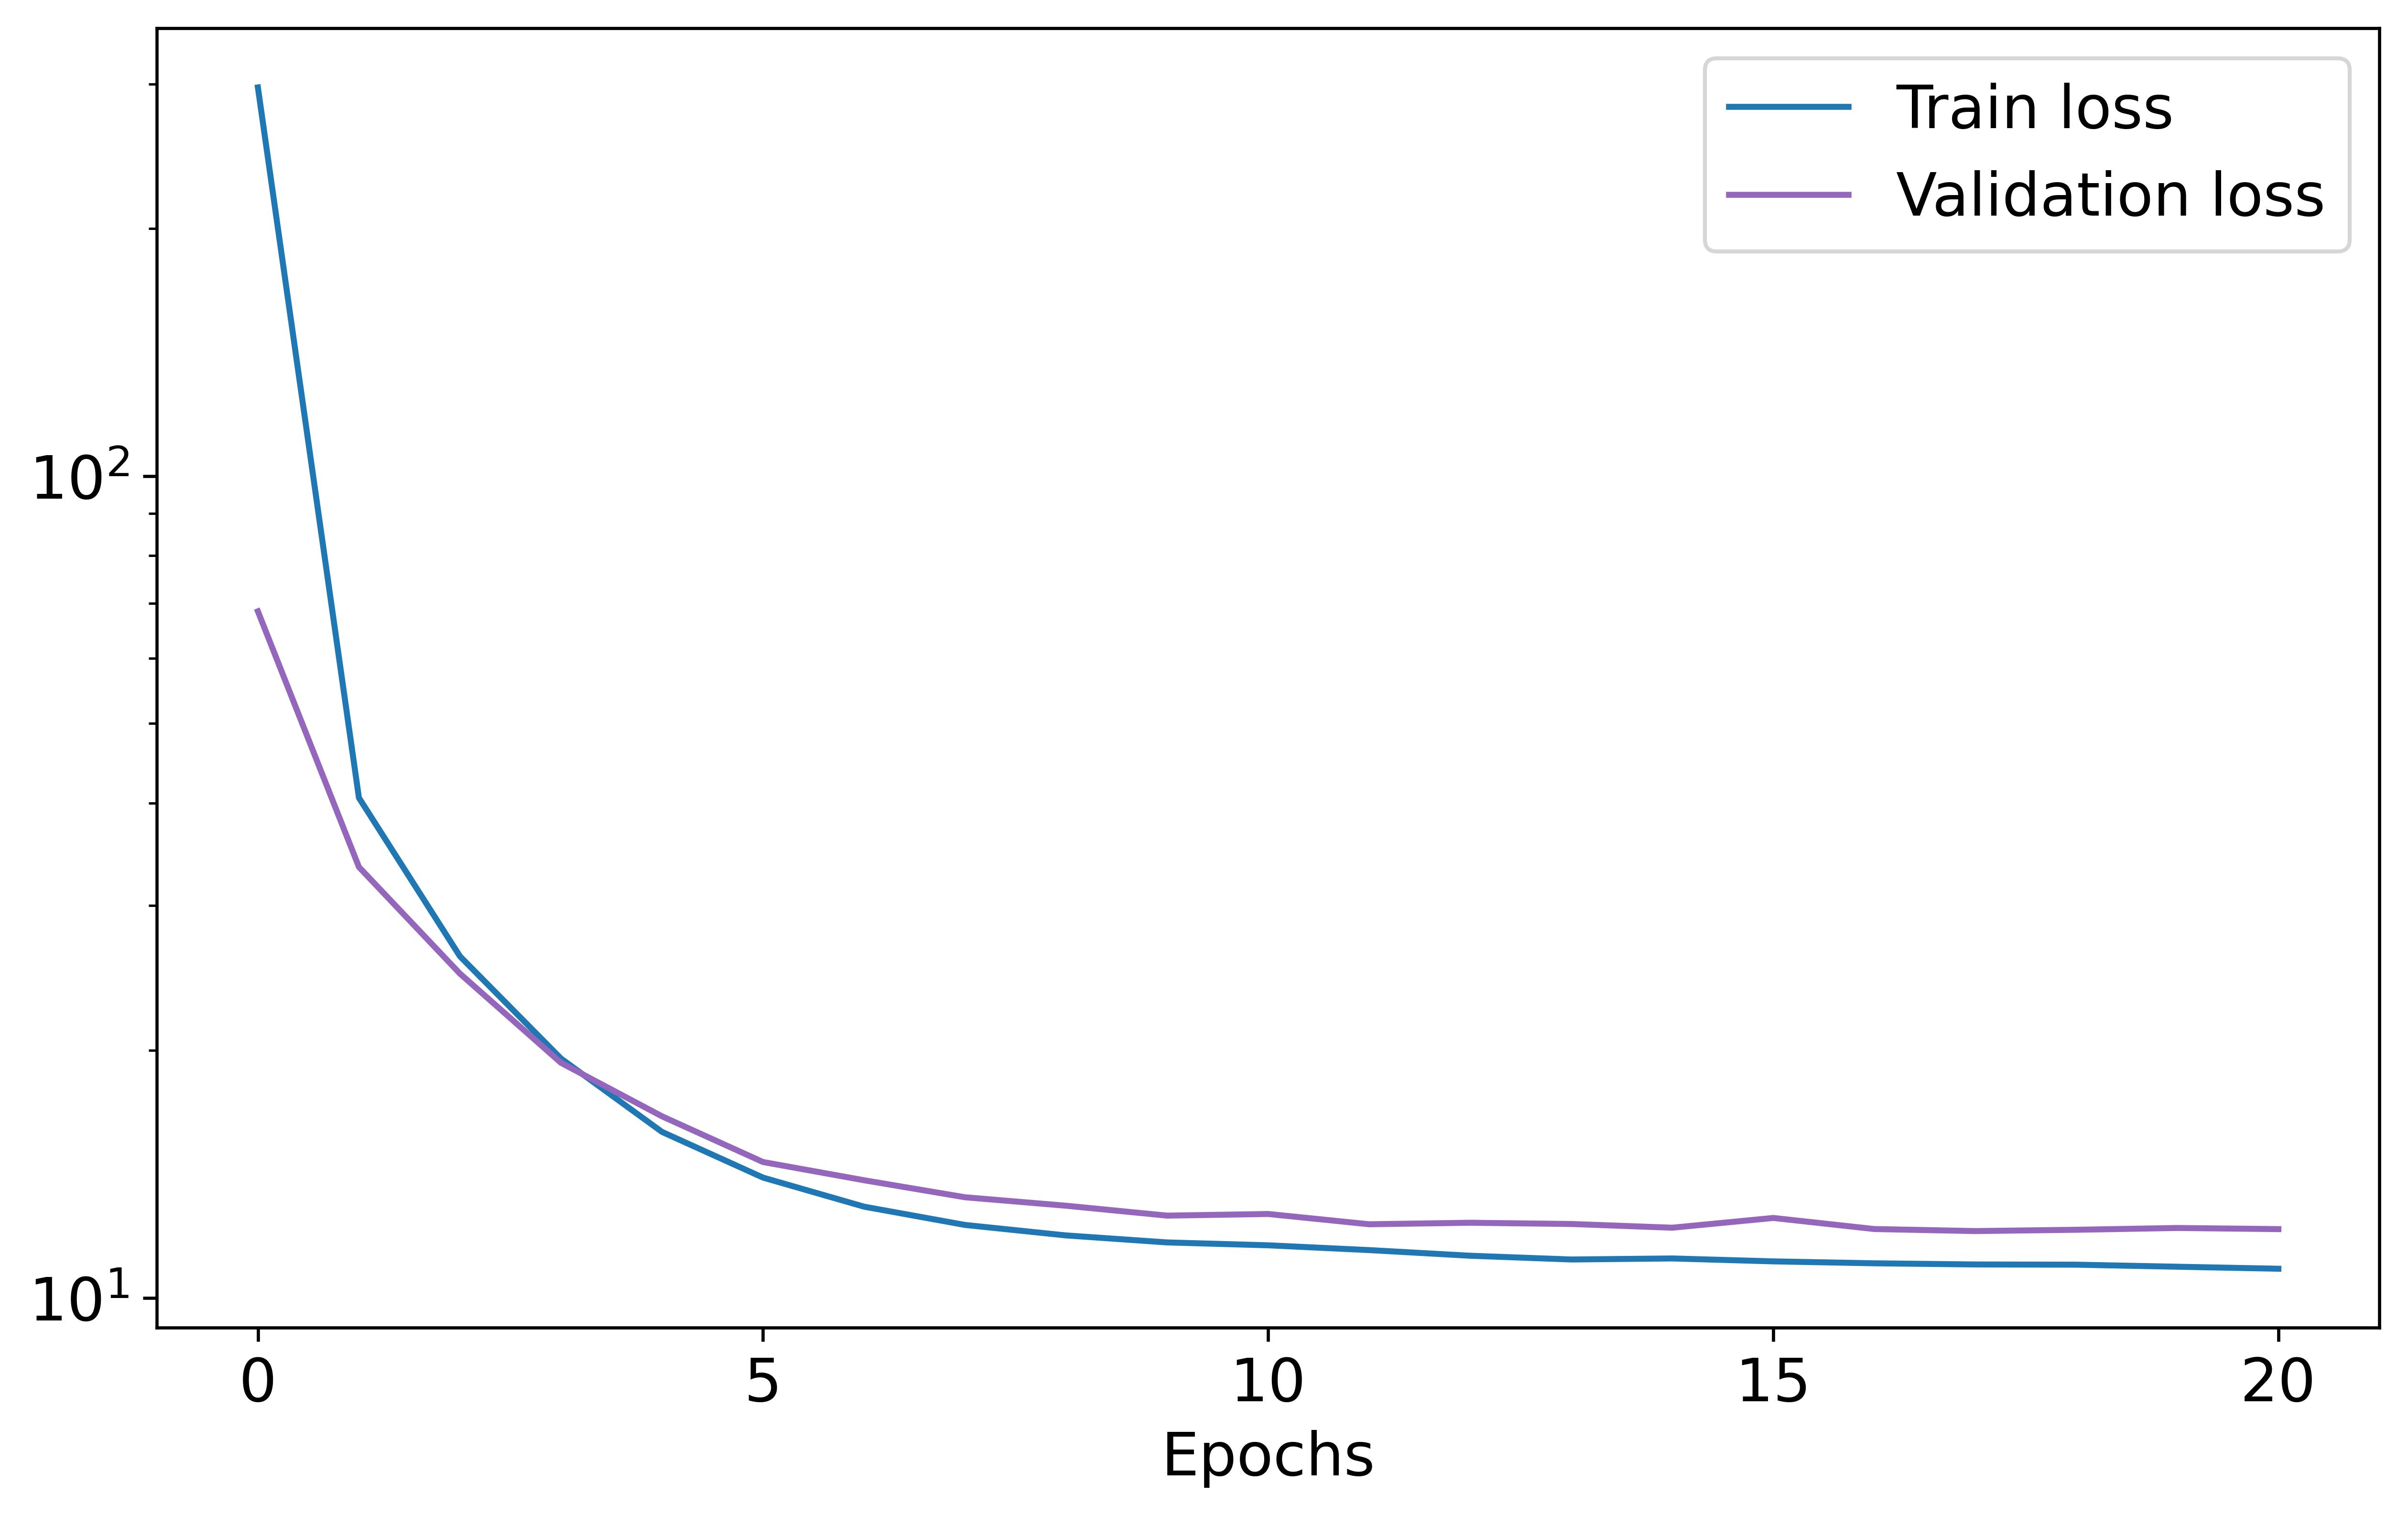
\includegraphics[width=.95\linewidth]{img/restrain.png}
	\captionof{figure}{ResNet training}
	\label{fig:Res}
\end{minipage}%
\begin{minipage}{.5\textwidth}
	\centering
	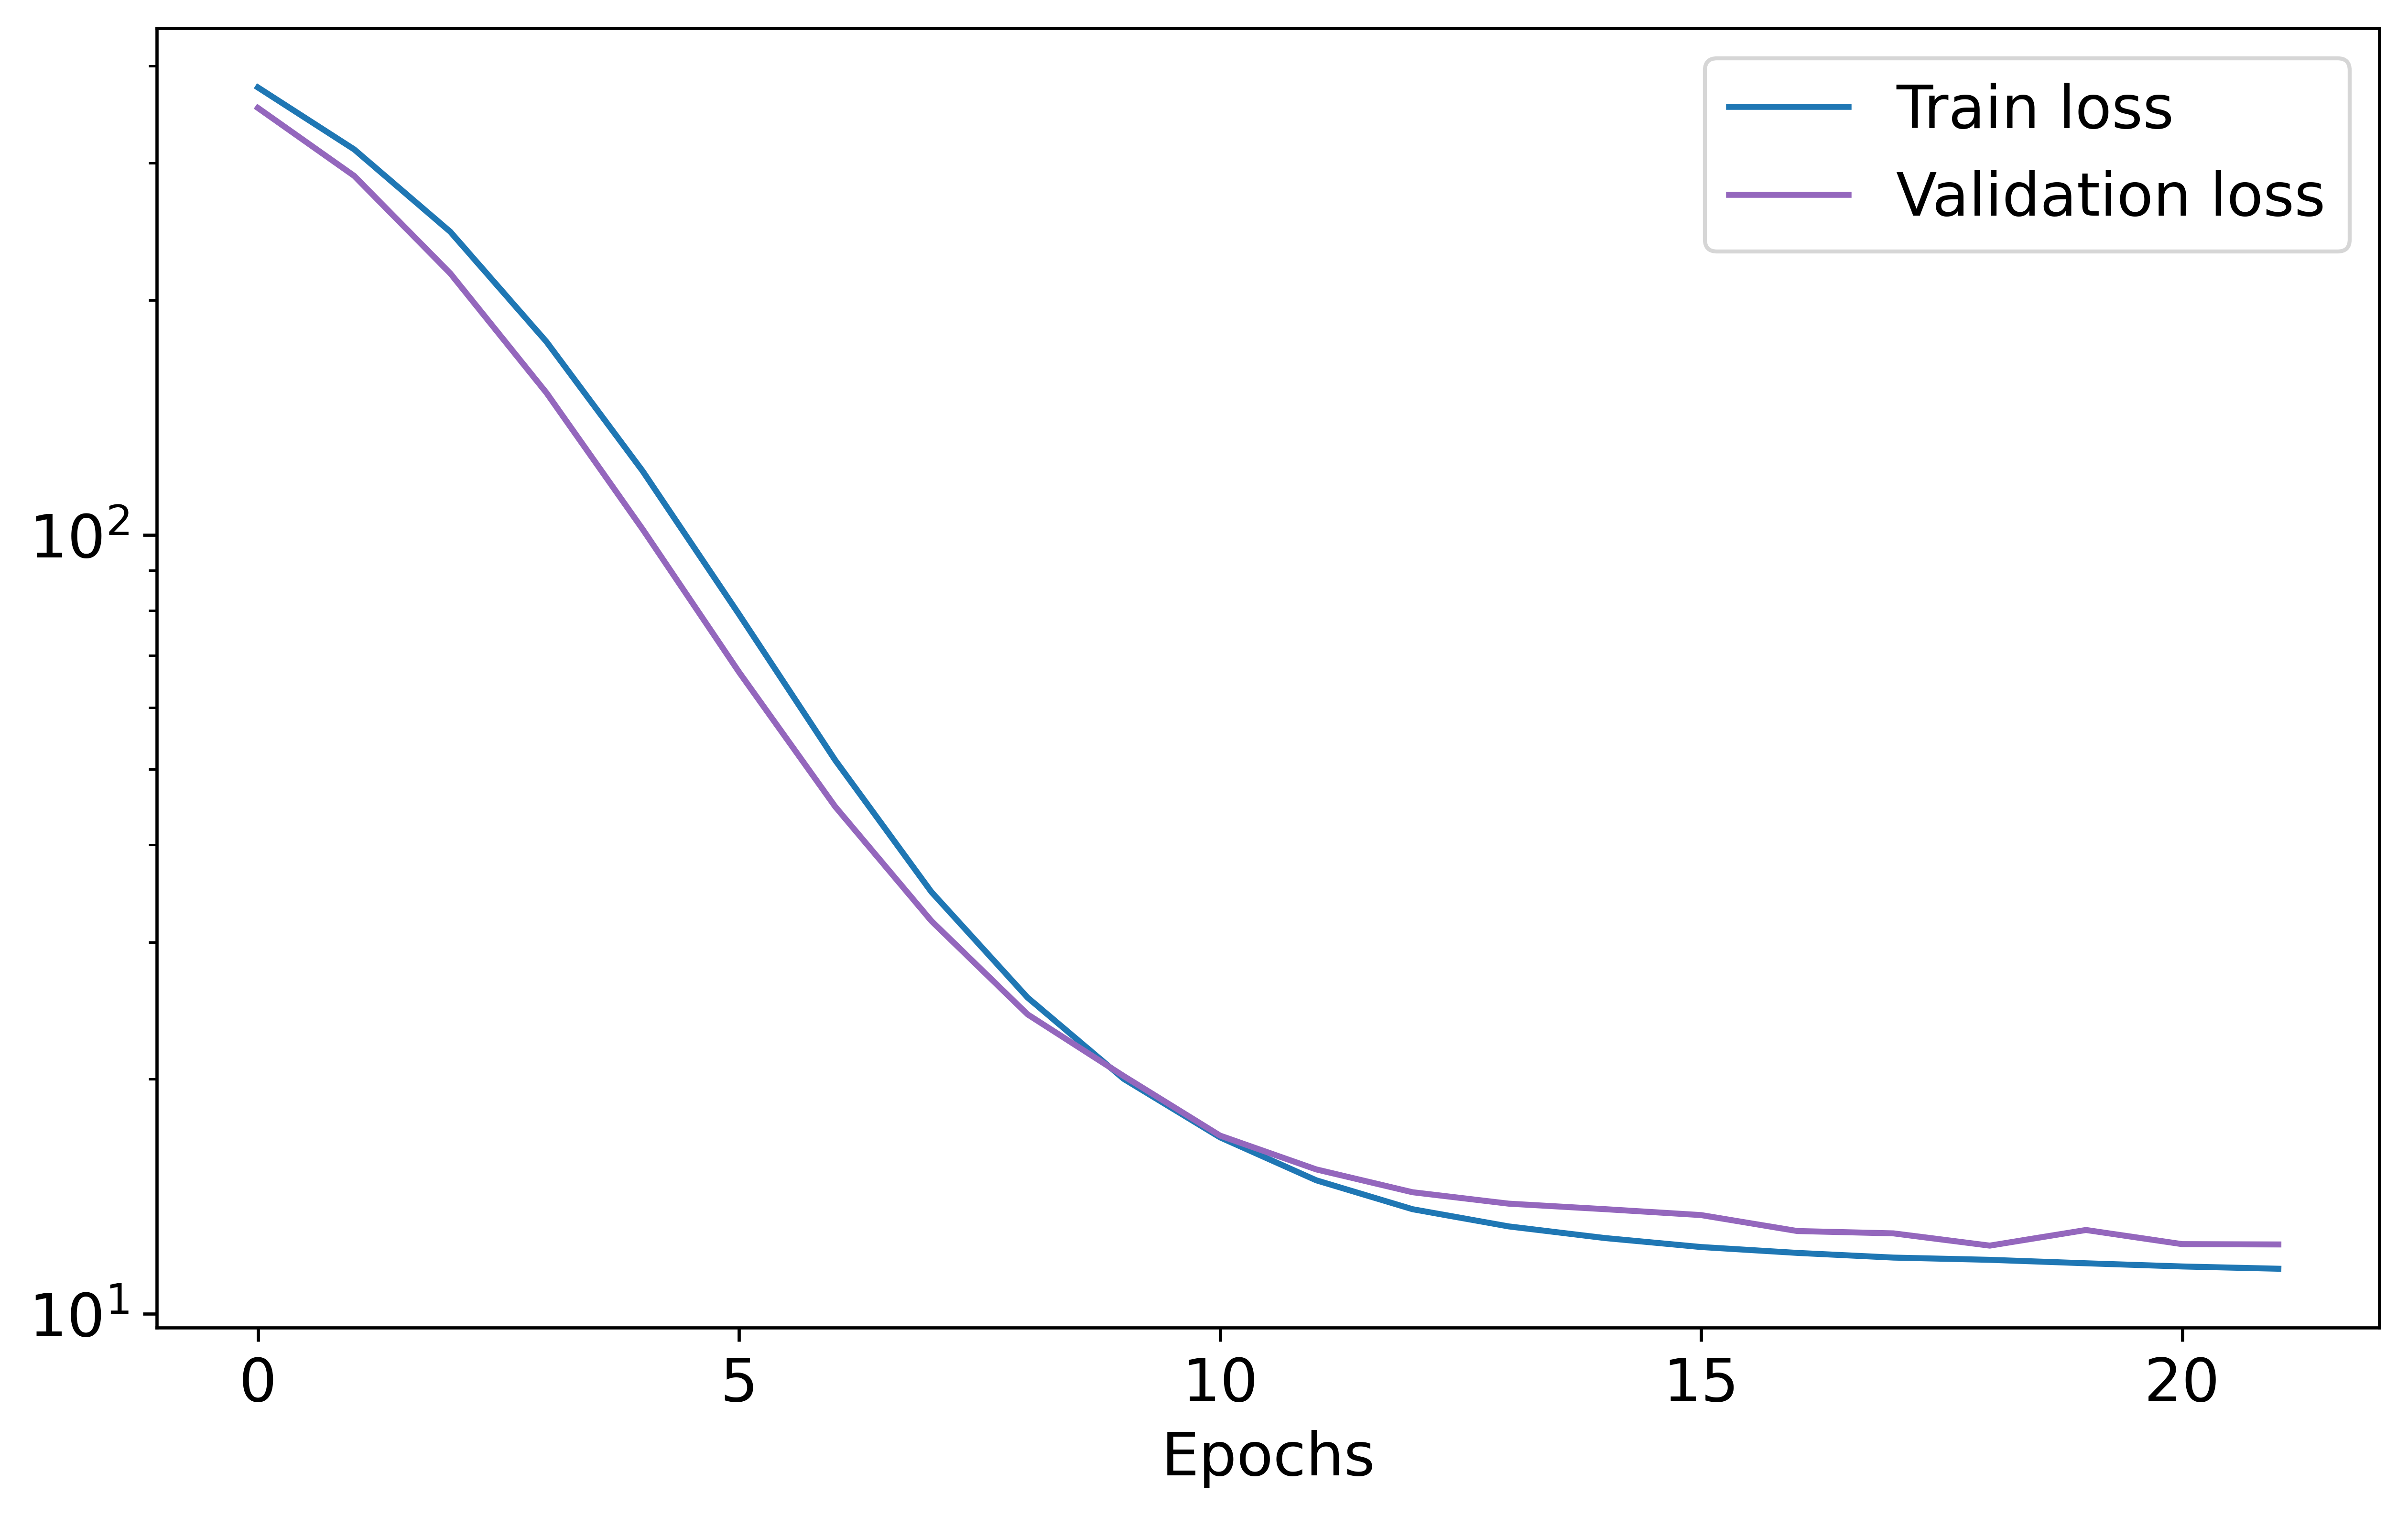
\includegraphics[width=.95\linewidth]{img/convtrain.png}
	\captionof{figure}{ConvNet training}
	\label{fig:Conv}
\end{minipage}
\end{figure}

\saut

Table \ref{tab:results} compares the RMSE obtained in the different situations: NWP, linear baseline and convolutional
multi-task network predicting each concerned variable one and two hours ahead. Not only are the multi-task
RMSE higher but they increase fast with the number of timesteps predicted.

\saut

Such results reveal that the underlying system has a linear behaviour: the neural networks tend to mimic
a linear model but is less good at it than a properly linear model. Considering the baselines' characteristics,
it is clear that all the models implemented actually mainly rely on the measurement
at time $t$ when predicting value at time $t + 1$. In other
words, the linear model doesn't manage to extract enough information from the rest of the input and the neural
networks don't fix this issue. Hence a linear behaviour too. In other words,
as they lack the ability to capture the
right information, all the investigated models almost boil down to persistence with bias correction.

\saut

Such limit is likely to come from the absence of spatial information within the inputs whereas weather is fundamentally
a time-space coupled system. Only a few NWP timeseries are not enough to convey a relevant 
part of the knowledge contained in the physical model used to make the predictions so that NWP correction cannot
be achieved this way.

\vspace{20px}

\begin{table}[htb]\centering
\begin{tabular}{ccccc}
\toprule
      Feature&NWP RMSE&Baseline RMSE&\multicolumn{2}{c}{Multi-task RMSE}\\\cmidrule{4-5}
      &	 &	&	Ouput 1	&Output 2\\ \midrule
      GHI	&40.70&61.03&	44.32&54.38\\
      $\mathrm W_{\mathrm x}$	&1.97&1.09&1.13&1.36\\
      $\mathrm W_{\mathrm y}$	&1.12&2.24&1.16&1.43\\
      \bottomrule
\end{tabular}
\caption{Multi-task models results}
\label{tab:results}
\end{table}

\section*{Conclusion and future work}

This paper is about considering multiple representations of a set of weather variables -- GHI, temperature, wind speed
and direction -- including both \emph{in-situ} measurements and model-based numerical predictions to
output local short-term predictions of such variables and apply them to renewable energy planning. This selection
of inputs brings to the model information on the future through NWP and accurate data on the past
through measurements and thus allows NWP correction.
Considering the relationships between the weather variables at stake and the similarity
between the different prediction tasks, three multi-task models were investigated and compared to linear baseline
models. The baselines showed encouraging performances, revealing that the chosen architecture could indeed
participate in NWP correction.
However, multi-tasks neural networks led to unexpectedly bad results and were unable to improve the baseline
performances. The main conclusion that can be drawn is that the implemented models don't manage to fully
benefit from the numerical predictions added value with respect to the observations.

\saut

The most promising perspective would be to take into account the space dimension, that is to say not to take as input
the timeseries of each variable at a specific location -- here Monaco -- but a grid of such values all around the
targeted place for each timestep.
As the adopted strategy focusing on NWP correction was in particular chosen to tackle the geographical resolution
of the numerical models, time-space models can be expected to bring more complete and useful information.
That would especially allow more sophisticated convolutional models.
It would also be interesting to investigate recurrent networks and particularly
LSTM which can learn short-term as well as long-term mechanisms. Yet, the main obstacle remains the amount of data
available which keeps from implementing deep networks.

\section*{Acknowledgements}

I would like to sincerely thank Philippe Blanc, Sébastien Travadel, Yves-Marie Saint-Drenan and Hadrien Verbois
for their availability, kind help and support.

\bibliographystyle{unsrt}
\bibliography{references}

\end{document}
